% -----------------------------------------------
% Template for ISMIR Papers
% 2015 version, based on previous ISMIR templates
% -----------------------------------------------

\documentclass{article}
\usepackage{ismir}
\usepackage{url}
\usepackage{cleveref}
\usepackage{cite}
\usepackage{brian}
\usepackage{graphicx}
\usepackage{booktabs}

% Title.
% ------
\title{Musical data augmentation}


% Single address
% To use with only one author or several with the same address
% ---------------
%\oneauthor
% {Names should be omitted for double-blind reviewing}
% {Affiliations should be omitted for double-blind reviewing}

% Two addresses
% --------------
%\twoauthors
%  {First author} {School \\ Department}
%  {Second author} {Company \\ Address}

% Three addresses
% --------------
\threeauthors
  {First author} {Affiliation1 \\ {\tt author1@ismir.edu}}
  {Second author} {\bf Retain these fake authors in\\\bf submission to preserve the formatting}
  {Third author} {Affiliation3 \\ {\tt author3@ismir.edu}}

% Four addresses
% --------------
%\fourauthors
%  {First author} {Affiliation1 \\ {\tt author1@ismir.edu}}
%  {Second author}{Affiliation2 \\ {\tt author2@ismir.edu}}
%  {Third author} {Affiliation3 \\ {\tt author3@ismir.edu}}
%  {Fourth author} {Affiliation4 \\ {\tt author4@ismir.edu}}

\begin{document}
%
\maketitle
%
\begin{abstract}
Predictive models for music annotation tasks are practically limited by a paucity of
well-annotated training data.
In the broader context of large-scale machine learning, the concept of ``data
augmentation'' --- supplementing a training set with carefully perturbed samples ---
has emerged as an important component of robust systems.
In this work, we develop a general software framework for augmenting annotated
musical datasets, which will allow practitioners to easily expand training sets
with musically motivated perturbations of both audio and annotations.
As a proof of concept, we investigate the effects of data augmentation on
the task of recognizing instruments in mixed signals.
\end{abstract}
%
\section{Introduction}
\label{sec:introduction}

% Main points to make:
%   1. music is complex, and needs big models
%       a. big models need big data
%       b. big (annotated) data is hard to come by

Musical audio signals contain a wealth of rich, complex, and highly structured
information.  The primary goal of content-based music information retrieval (MIR) is to
analyze, extract, and summarize music recordings in a human-friendly
format, such as semantic tags, chord and melody annotations, or structural boundary
estimations.  Modeling the vast complexity of musical audio seems to require large, 
flexible models with many parameters.
By the same token, estimating the parameters of complex statistical models often requires
a large number of samples: big models require big data.

Within the past few years, this phenomenon of increasing model complexity has been 
observed in the computer vision literature.  Currently, the best-performing models for 
recognition of objects in images exploit two fundamental properties to overcome the 
difficulty of fitting large, complex models: access to large quantities of annotated data, 
and identifying label-invariant data transformations~\cite{krizhevsky2012imagenet}.
The benefits of large training collections are obvious, and unfortunately, difficult to
carry over to most musical annotation tasks due to the complexity of the label space and
need for expert annotators.  However, the idea of generating perturbations of a training
set --- known as \emph{data augmentation} --- can be readily adapted to musical tasks.

%   2. in images:
%       a. data augmentation has proven useful in vision.
%       b. general idea: perturb your data such that the features change, but the labels
%       don't
%       c. rotations, reflections, contrast normalization, affine transformations
Conceptually, data augmentation consists of the application of one or more deformations to
a collection of (annotated) training samples.
Data augmentation is motivated by the observation that a learning algorithm may
generalize better if it is trained on instances which have been perturbed in ways 
which are irrelevant to their labels.
Some concrete examples of deformations drawn from computer vision include translation,
rotation, reflection, and scaling.
These simple operations are appealing because they typically do not affect the target 
class label: an image of a cat still contains a cat, even when it is flipped upside-down.
%although the situation may be more complex for concepts which are not reflection-invariant,
%such as in optical character recognition.  Consequently, practitioners must exercise some
%caution when applying data augmentation techniques to ensure that the correct invariances
%are maintained.

More generally, we may consider deformations which apply not only to the observable
features, but the labels as well.
Continuing with the image example, if an image is rotated by some angle, 
then any pixel-wise label annotations (\eg, bounding boxes) should also be rotated by
that angle.
This observation opens up several interesting possibilities for musical applications, in
which the target concept space typically exhibits a high degree of structure.
As a musical analog to the image rotation example, time-stretching an audio track 
should induce a dilation of time-keyed annotations boundaries (\eg, chord or instrument
activation timings)~\cite{mauch2013audio}.

Moreover, many natural, musically-inspired deformations
would not only change the position of annotations, but the annotation
\emph{values} themselves.
For instance, if a track has tempo annotations, any time-stretching deformations should
be applied to the annotations as well.
Similarly, pitch-shifting a track should induce transpositions of annotated fundamental
frequency curves, and if the transposition is sufficiently large, chord labels or symbolic 
annotations may change as well.
It follows that successful use of data augmentation in MIR may require
substantially more careful implementations and transformation algorithms than are currently
in use in other domains.

%   3. but data augmentation is more difficult in music than in images
%       a. the output space is much more complex than simple tags
%       b. it's not obvious which variations preserve output structure
%       c. simple example: time-stretching will move annotation boundaries
%       d. complex example: pitch-shifting will deform chord labels

\subsection{Our contributions}
% 1. develop a generic framework for synchronously manipulating audio and annotations
% 2. investigate the effects of simple deformations on the problem of musical instrument recognition
In this work, we describe a software architecture for applying data augmentation to music
information retrieval tasks.\footnote{For anonymity purposes, the name of the software
    described here is redacted throughout the text.  This will be changed in the final
draft, and download links will be provided.}
The system is designed to be simple, modular, and
extensible. The design enables practitioners to develop custom deformations, and combine
multiple simple deformations together into pipelines which can generate large volumes of
reliably deformed, annotated music data.  The proposed system is built on top of
JAMS~\cite{humphreyjams}, which provides a simple container for accessing and
transporting multiple annotations for a given track.

As a proof of concept, we apply the proposed data augmentation architecture to the
task of recognizing instruments in mixed signals, and demonstrate that simple
manipulations can yield improvements in accuracy.

\section{Related work}

% 1. it's common to engineer systems to attempt to resolve symmetries in the input,
%       eg, chroma features are engineered to be approximately invariant to timbre and octave
%       some authors suppress the 0th mfcc to get loudness invariance
The first step in developing a solution to an MIR problem is often to
design features which discard information thought to be irrelevant to the target
concept.  For example, chroma features are designed to capture pitch class information
and suppress timbre, loudness, or octave height~\cite{muller2011chroma}.
Similarly, many authors interested in modeling timbre
use Mel-frequency cepstral coefficients (MFCCs) and discard the first component to
achieve invariance to loudness~\cite{pampalk2004matlab}.
This general strategy makes intuitive sense, but it carries many limitations.
First, it is not necessarily easy to identify all relevant symmetries the
data: if it was, the modeling problem would be essentially solved.
Second, even if such properties are easy to identify, it may still be difficult to
engineer appropriately invariant features without discarding potentially useful
information.  For example, 2-D Fourier magnitude coefficients achieve invariance to
time- and pitch-transposition, but discard phase coherence~\cite{ellis2012large}.

%   but there are some drawbacks:
%       a. it's not easy to identify *all* relevant symmetries
%       b. even if it was, it might not be easy to engineer an invariant feature
%       c. and you might accidentally discard useful information in the process
%
%   alternatively:
%       we can use bigger models
%       learn the appropriate invariances from statistics.
%       but this takes a lot of (annotated) data, which we usually don't have
%
%
As an alternative to custom feature design, some authors advocate learning or optimizing
features directly from the data~\cite{humphrey2012moving}.
Not surprisingly, this approach typically requires large model architectures, and
much larger (annotated) data sets than had previously been used in MIR research.  
Due to the high cost of acquiring annotated musical data, it has so far been difficult to
apply these techniques in most MIR tasks.
While some authors have advocated leveraging unlabeled data to ``pre-train'' feature
representations~\cite{dieleman2011audio}, 
recent studies have shown that comparable or better performance can be
achieved with random initialization and fully supervised training~\cite{glorot2011deep,zeiler2013rectified}.
Our goal in this work is to provide data augmentation tools which may ease the burden of 
sample complexity, and make data-driven methodology more accessible to the MIR community.

% 1. augmentation is not new, but it hasn't been done systematically.
%   eg, chroma rotation for key-invariance in chord quality or mode
%   synthetic mixtures of clean signals
%   perturbations of the labels ``target smearing''
%
Specific instances of data augmentation can be found throughout the MIR literature,
though they are not often identified as such, nor are they treated systematically 
in a unified framework.
For example, it is common to apply circular rotations to chroma features
to achieve key invariance when modeling chord quality~\cite{lee2008acoustic}.
Alternately, synthetic mixtures of monophonic instruments have been used
to generate non-trivial examples when training polyphonic transcription
engines~\cite{kirchhoff2012multi}.
At the other end of the spectrum, some authors leave the audio content unchanged and
only modify labels during training, as exemplified by the \emph{target smearing}
method of Ullrich~\etal\ for training structural boundary
detectors~\cite{ullrich2014boundary}.

% finally, recent studies have investigated stability of models by evaluating on degraded signals:
%   but it's not clear that the degraded signals resemble the distribution of naturally occurring sounds
%   our goal is different: train on degraded signals, and evaluate on unmodified signals
%
%
Finally, recent studies have used degraded signals to evaluate the stability of
existing methods for MIR tasks.
The Audio Degradation Toolbox (ADT) was developed for this purpose, and was used
to measure the impact of naturalistic deformations of audio on several tasks, including
beat tracking, score alignment, and chord recognition~\cite{mauch2013audio}.
Similarly, Sturm and Collins proposed the ``Kiki-Bouba Challenge'' as a way to determine
whether statistical models of musical concepts actually capture the defining
characteristics of the concept (\eg, genre), or are over-fitting to spurious
correlations~\cite{sturmkiki}.

In both of the studies cited above, models are fit to unmodified data, and evaluated in
degraded conditions under the control of the experimenter.
Data augmentation provides the converse of this setting: models are fit to degraded data,
and evaluated on unmodified examples.  The distinction between the two approaches is
critical.  The former attempts to measure the robustness of a system under synthetic
conditions, while the latter attempts to improve robustness by \emph{training} under
synthetic conditions. Note that with data augmentation, the evaluation set is left
untouched by the experimenter, so the resulting comparisons are unbiased with respect
to the underlying distribution from which the data are sampled.  While this does not
directly measure robustness of the resulting system, it has been observed  
that data augmentation can improve generalization~\cite{krizhevsky2012imagenet,he2015delving}.


\section{Data augmentation architecture}

% 1. because of the complex structure of annotations, we need to be careful
%   a. annotations aren't just track-level, but generally time-keyed
%   b. simple deformations can change annotations, such as chord labels or pitch
%   frequencies
%
% 2. why not use the audio degradation toolbox?
%   a. we'd like to be more extensible, support annotation-dependent deformations
%   b. support multiple annotations per-track
%   c. want the ability to embed history within the annotations for reproducibility
%   purposes
%   d. closer integration with python libraries for machine learning (eg theano)
%
% 3. we developed a generic, plugin-oriented architecture for doing musical data augmentation
%   a. hooks into JAMS, and inherits validation/schema.
%   b. also makes it easy to modify all annotations for a given track in one shot.
%   c. allows the developer to register a deformation against different types of data
%       eg, a ``pitch-shift'' deformer implements an audio deformation, pitch annotation modification, and
%       chord/key manipulators
%   e. modules can be chained or skipped in a pipeline, similar to sklearn feature extractors
%       pipelines can be serialized, stored, shared, and reimplemented easily
%   f. full history of modification state is preserved within the output JAMS sandbox, so the results are
%   documented and reproducible
%       this includes all random state
%   g. deformations can be stochastic, and potentially generate infinite streams of randomized data
%       more generally, a deformer object can implement its own state transition logic
%       using python iterators makes this simple, self-contained, and memory-efficient
Our implementation takes substantial inspiration from the Audio Degradation
Toolbox~\cite{mauch2013audio}.  In principle, the ADT can be used directly
for data augmentation simply by applying it to the training set rather than test set.
However, we opted for an independent, Python-based implementation for a variety of
reasons as detailed below.

% 1. object-oriented design
%   simple, reusable components that are easy to modify and extend
%
First, Python enables object-oriented design, allowing for structured,
extensible, and reusable code.  This in turn facilitates a simple interface shared across
all \emph{deformation objects}, and makes it easy for practitioners to combine existing
deformations, or implement new transformations with minimal effort.

% 2. leverage jams as a container
%   transform all annotations for an object at once
%       -> everything stays in sync easily
%   store the transformation properties within the jams sandbox
%       -> reproducibility, provenance
%   the jams sandbox can store the audio and other intermediate features
%       ->
%   allow deformers to apply different transformations to different types of annotations
%       implemented as simple callbacks registered against annotation types or patterns
%

Second, we use JAMS objects~\cite{humphreyjams} to contain and transport all
annotations and audio content for a given track.
This simplifies the tasks of maintaining synchronization between audio and annotations,
and implementing task-dependent annotation deformations.  Moreover, we take
advantage of JAMS meta-data fields to provide data provenance and facilitate
reproducibility.

% 3. use familiar design paradigms
%   take inspiration from the Transformer and Pipeline paradigms of scikit-learn
%
Finally, we borrow familiar software design patterns from the SciKit-Learn
package~\cite{buitinck2013api}, such \emph{transformers}, \emph{pipelines}, 
and model serialization.  These simple building blocks allow
practitioners to quickly and easily assemble complex data augmentation pipelines 
from small, conceptually simple components.

% Give a figure illustrating how deformers work
%   deformer
%       generates states as a function of a jam
%       registers callbacks against annotation types
%   pipeline
%       chains deformers together
%   bypass
%       make a deformer optional

In the remainder of this section, we will describe each of these
properties in more detail.  Without loss of generality, we will assume that an
annotation (\eg, instrument activations or semantic tags) is encoded as a collection of
tuples: \emph{(time, duration, value, confidence)}.
Note that instantaneous events can be represented as having zero duration, while
track-level annotations have full-track duration.  The \emph{value} field will depend on
the annotation type, and may encode strings, numeric quantities, or fully structured
objects.

\subsection{Deformation objects}

At the core of our implementation is the concept of a \emph{deformation object}.
A deformation object implements one or more \emph{transformation} methods, each of which
applies to audio data, meta-data, or annotations.
Parameters of the deformation are shared through a \emph{state} object $S$:
For example, $S$ might contain the speed-up factor of a
time-stretch operation, or the number of semi-tones in a pitch-shift.  
Each transformation method thus takes as input a pair $(S, x)$ and
returns the suitably transformed audio, meta-data, or annotation $x'$.
This decoupling of the deformation object's instantiation from
its state allows multiple tracks to be processed in parallel by the same object.
Moreover, as described in \Cref{sec:reproducibility}, it promotes reproducibility 
by making state objects re-usable.

Data augmentation often requires sweeping or randomly sampling a set of deformation 
parameters, and instantiating a separate deformation object for each parameterization 
would be woefully inefficient.
To streamline this process, deformation objects must provide \emph{state generators},
which may implement arbitrary state transition logic to produce a sequence of 
state objects.  This is accomplished efficiently via Python's \emph{generator}
functionality.

Finally, deformation objects may register transformation functions against the 
\emph{type} of an annotation, as described by regular expressions.
During execution, the JAMS object is queried for all annotations matching the specified
expression, and the results are processed by the corresponding transformation method.
For example, the expression ``\texttt{.*}'' matches all annotation types, while 
``\texttt{chord.*}'' matches only chord-type annotations.
These patterns need not be unique or disjoint, though care must be taken
to ensure consistent behavior.
Deformations are always applied following the order in which they are registered, 
and we encourage the convention that patterns be registered in order of decreasing
generality.

The abstract transformation algorithm is described in \Cref{alg:transformation}.
For each state $S$, the input data $J$ is copied, transformed into $J'$, and yielded 
back to the caller. 
Each $J'$ can then be saved off to disk, provided as a sample to an iterative learning 
algorithm, or passed along to another deformation object in a pipeline for further processing.
When all subsequent processing of $J'$ has completed, \Cref{alg:transformation} may resume
computation at line~10 and proceed to the next state at line~2.

\begin{algorithm}[t]
\caption{Abstract transformation pseudocode\label{alg:transformation}}
\begin{algorithmic}[1]
    \Require{Deformation object $D$, JAMS object $J$}
    \Ensure{Sequence of transformed JAMS objects $J'$}
    \Function{$D$.transform}{$J$}
    \For{states $S \in D.\Call{states}{J}$}
        \State{$J' \leftarrow \Call{copy}{J}$}
        \State{$J'.\text{audio} \leftarrow D.\Call{audio}{S, J'.\text{audio}}$}
        \State{$J'.\text{meta}\leftarrow D.\Call{metadata}{S, J'.\text{meta}}$}
        \For{transformations $g$ in $D$}
            \For{annotations $A \in J'$ which match $g$}
                \State{$J'.A \leftarrow g(S, A)$}
            \EndFor{}
        \EndFor{}
        \State{$J'.\text{history} \leftarrow \Call{Append}{J'.\text{history}, S}$}
        \State{\textbf{yield} $J'$}
    \EndFor{}
    \EndFunction{}
\end{algorithmic}
\end{algorithm}


\subsubsection{Example: randomized time-stretching}
To illustrate the deformation object interface, we will describe the implementation of a 
randomized \emph{time-stretch} deformation object.
In this case, each \emph{state} object contains a single quantity: the stretch factor $f$.
\Cref{alg:timestate} illustrates the state-generation logic for a randomized
time-stretcher, in which some $n$ examples are generated by sampling $f$ uniformly at
random from an interval $[f_-, f_+]$.\footnote{The parameters $n, f_-, f_+$ are actually
    properties of the deformation object, but are listed here as method parameters to
simplify exposition.}

The JAMS object $J$ over which the deformations will be applied is also provided as input 
to the state generator.  Though not used in this example, it allows the state generator
to pre-compute quantities of interest, such as track duration 
 --- which is necessary to ensure well-defined outputs from target-smearing deformations --- 
or tuning estimates, which are used by pitch-shift deformations to 
determine when a shift is large enough to 
alter note labels.

Once a state $S$ has been generated, the $\Call{audio}$ deformation method
--- $D.\Call{audio}{S, J.\text{audio}}$ --- 
applies the time-stretch to the audio signal, which is stored within the
JAMS sandbox upon instantiation.\footnote{The \emph{sandbox} provides unstructured
storage space within a JAMS object, which is used in our framework as a scratch space for
audio signals.}  Similarly, track-level meta-data can be modified by the $\Call{metadata}$
method.  In this example, time-stretching will change the track duration, which is recorded
in the JAMS meta-data field.

Next, a generic \emph{annotation} deformation would be registered to the pattern
``\texttt{.*}'' and apply the stretch factor to all \emph{time} and \emph{duration}
fields of all annotations.  This deformation would leave the annotation
\emph{values} untouched, since not all annotation types have time-dependent values.

Finally, any annotations whose \emph{value} fields depend on time, such as \emph{tempo},
can be modified directly by registering the transformation function against the
appropriate type pattern, \eg, ``\texttt{tempo}''.  Other time-dependent type
deformations would be registered separately as needed.

\begin{algorithm}[t]
    \caption{Randomized time-stretch state generator\label{alg:timestate}}
    \begin{algorithmic}[1]
        \Require{JAMS object $J$, number of deformations $n$, range bounds $(f_-, f_+)$}
        \Ensure{Sequence of states $S$}
        \Function{RandomStretch.states}{$J, n, f_-, f_+$}
            \For{$i$ in $1, 2, \dots, n$}
            \State{Sample $f \sim { }_U[f_-, f_+]$}
            \State{\textbf{yield} $S=\{f\}$}
            \EndFor{}
        \EndFunction{}
    \end{algorithmic}
\end{algorithm}

The time-stretching example is simple, but it serves to illustrate the flexibility of 
the architecture.
It is straightforward to extend this example into more sophisticated deformations 
with structured state generators to sweep over deterministic parameter grids.
For example, an additive background noise deformation could be parameterized by 
a collection of noise sources and a range of gain parameters, and 
generate one example for each unique combination of source and gain.

\subsection{Pipelines and bypasses}
\Cref{alg:transformation} describes the process by which a deformation object turns a
single annotated audio example into a sequence of deformed examples.  If we were
interested in experimenting with only a single type of augmentation (\eg, time stretching),
this would suffice.  However, some applications may require combining or cascading
multiple types of deformation, and we prefer a unified interface that obviates the
need for customized data augmentation scripts.

Here, we draw inspiration from SciKit-Learn in defining \emph{pipeline}
objects.  The general idea is simple: two or more deformation objects can be chained
together, and treated as a single, integrated deformation object.  This functionality
mimics that of the SciKit-Learn \emph{Transformer} pipeline,\footnote{\url{http://scikit-learn.org/stable/modules/generated/sklearn.pipeline.Pipeline.html}} except that rather
than applying a composition of one-to-one mappings, deformation pipelines
compose functions in a one-to-many fashion.  More precisely, for a deformation pipeline
$P$ composed of $k$ stages:
\[
P = (D_1, D_2, \dots, D_k),
\]examples are generated by a depth-first traversal of the
cartesian product of the corresponding state spaces
\[
\Sigma_P = \Sigma_1 \times \Sigma_2 \times \cdots \times \Sigma_k.
\]
A single input example produces $|\Sigma_P|=\prod_{i=1}^k |\Sigma_i|$ outputs.
By using generators rather than explicit lists of states, 
we ensure that only $k$ examples are ever in memory at any time.
In most cases, $k$ is much smaller than $|\Sigma_P|$, which provides substantial
improvements to memory efficiency.

Finally, we introduce the \emph{bypass} object, which is used to mark
individual pipeline stages as optional.
Bypasses are useful when it is difficult to encode a special \emph{no-op} 
state within a deformation object, such as the randomized time-stretch 
example listed as \Cref{alg:timestate}.
The internal logic of a bypass object is simple: first, pass the input directly through
unmodified, and then generate samples from the contained deformation object as usual.
Bypasses can be used to ensure that the original examples are propagated through the
pipeline unscathed, and the resulting augmented data set is a strict superset of the
clean data.

\subsection{Reproducibility and data provenance}
\label{sec:reproducibility}
When modifying data for statistical modeling purposes, maintaining transparency is of
utmost importance to ensure reproducibility and accurate interpretation of results.
This ultimately becomes a question of data provenance~\cite{buneman2000data}: a record of
all transformations should be kept, preferably attached as closely as possible to the data.
Rather than force practitioners to handle book-keeping, we automate the process from within
the deformation engine.
This is accomplished at line~9 of \Cref{alg:transformation} by embedding the
\emph{state} object $S$ (and, in practice, the parameters used to construct the
deformation object $D$) within the JAMS object after each deformation is applied.
Each $J'$ generated at line~10 thus contains a full transactional history of all
modifications required to transform $J$ into $J'$.
For this reason, stochastic deformations are designed so that all randomness is contained
within the state generator, and transformations are all deterministic.

In addition to facilitating reproducibility, maintaining transformation provenance allows
practitioners to generate a wide range of deformations up front, and then later filter the
resulting objects.  As a result, it is straightforward to generate a suite of experiments
over different subsets of data augmentation parameters.

To further facilitate reproducibility and sharing of experimental designs, the proposed
architecture supports \emph{serialization} of deformation objects and pipelines into a 
simple, human-readable JavaScript object notation (JSON) format.
Once a pipeline has been constructed, it can be exported, edited as plain text, shared,
and reconstructed.  This feature also simplifies the
process of applying several different sets of deformation parameters, and eliminates the
need for writing a custom script for each setting.

\section{Example application: multi-instrument recognition}

To illustrate the data augmentation process, we applied it to the task of instrument
recognition in mixed audio signals.  For this task, we used the MedleyDB dataset, which
consists of 122 tracks, spanning a variety of genres and
instrumentations~\cite{bittner2014medleydb}.  Each track is annotated with time-varying
instrument activation functions, which are thresholded to provide a set of active
instruments at each point in time.
Because of the relatively small sample size, we limit
the experiment to cover only the 15 most frequently used (by track) instruments, as
listed in \Cref{medleytags}.

\begin{table}
\caption{The 15 most frequently used instrument labels in MedleyDB.\label{medleytags}}
\centering
\small
    \begin{tabular}{lr}
        \toprule
        Instrument & Number of tracks\\
        \midrule
        drum set                    & 65\\
        electric bass               & 64\\
        piano                       & 42 \\
        male singer                 & 38 \\
        clean electric guitar       & 37\\
        vocalists                   & 27\\
        synthesizer                 & 27\\
        female singer               & 25\\
        acoustic guitar             & 24\\
        distorted electric guitar   & 21\\
        auxiliary percussion        & 18\\
        double bass                 & 16\\
        violin                      & 14\\
        cello                       & 11\\
        flute                       & 11\\
        \bottomrule
    \end{tabular}
\end{table}

For evaluation purposes, each track is split into one-second clips.
The system is then tasked with recognizing the instruments active within each clip.

\subsection{Data augmentation}

The data augmentation pipeline consists of four stages:

\begin{description}
    \item[Pitch shift] by $n \in \{-1, 0, +1\}$ semitones.
    \item[Time stretch] by a factor of $f \in \left\{ 2^{-1/2}, 1.0, 2^{1/2}\right\}$.
    \item[Background noise (bypass)] under three conditions:
        subway,\footnote{\url{https://www.freesound.org/people/jobro/sounds/112252/}}
        crowded concert hall,\footnote{\url{https://www.freesound.org/people/klankbeeld/sounds/171317/}}
        and night-time city noise.\footnote{\url{https://www.freesound.org/people/inkhorn/sounds/231870/}}
        The latter three were linearly mixed with random weights drawn uniformly
        $\alpha \sim { }_U[0.1, 0.4]$.
    \item[Dynamic range compression (bypass)] under two settings drawn from the {Dolby E}
        standards~\cite{dolbyE}: \emph{speech},
        and \emph{music~(standard)}.
\end{description}

Pitch-shift and time-stretch operations were performed by Rubberband~\cite{rubberband}, and dynamic range
compression was performed by sox~\cite{sox}.
Note that the first two stages include no-op parameter settings $n=0$ and $f=1$.  We use
bypasses on the final two stages to ensure that all combinations of augmentation are
present in the final set.

Combining all stages of the pipeline produces {$3\times 3\times 4\times 3 = 108$} variants of each input track.  To
simplify the experiments, we only compare the cumulative effects of the above
augmentations.  This results in five training conditions of increasing complexity:
\begin{description}
    \item[(N)] no augmentation,
        \vspace{-.5\baselineskip}
    \item[(P)] pitch shift,
        \vspace{-.5\baselineskip}
    \item[(PT)] pitch shift and time stretch,
        \vspace{-.5\baselineskip}
    \item[(PTB)] pitch shift, time stretch, and background noise,
        \vspace{-.5\baselineskip}
    \item[(PTBC)] all stages.
\end{description}

\subsection{Acoustic model}

% Input features:
%   CQT at 36 bpo, ranging from C3 to C8 => 216 bins, 512-frame hop at 22KHz
%   sample patches of 44 frames ~= 1.02s
%   logamplitude clipped to -80dB
%
%   CQT features enable 2d-convolution for pitch-invariant feature extraction
%   log scaling gives us relative amplitude invariance
%

The acoustic model used in these experiments is a deep convolutional network.
The input to the network consists of log-amplitude, constant-Q spectrogram patches extracted with librosa~\cite{librosa}.
Each example spans approximately one second of audio, corresponding to 44 frames at a hop length of 512 samples and sampling rate of $22050$~Hz.
Constant-Q spectrograms cover the range of C3 ($65.41$~Hz) to C9 ($4186$~Hz) at 36 bins
per octave, resulting in time-frequency patches $X \in \R^{216\times44}$.
Instrument activations are aggregated into a single binary label vector, such that an instrument is deemed active if its on-time within the sample exceeds 0.25 seconds.

Importantly, constant-Q representations are linear in both time and pitch, a property that can be exploited by convolutional neural networks to achieve translation invariance.
Thus a four-layer model is designed to estimate the presence of zero or more instruments in a time-frequency patch.
Formally, an input, $X$, is transformed into an output, $Z$, via a composite nonlinear
function $\mathcal{F}(\cdot \given \Theta)$, given a parameter set $\Theta$.
This is achieved as a sequential cascade of $L=4$ operations, $f_\ell(\cdot \given
\theta_\ell)$, referred to as \emph{layers}, the order of which is given by $\ell$:
\begin{equation}
\label{eq:layers}
Z = \mathcal{F}(X \given \Theta) = f_{L}(  ... f_2(f_1(X \given \theta_1) \given \theta_2) )
 \given \theta_{L})
\end{equation}
% \noindent Here, $\mathcal{F} = \{f_1, f_2, ... f_{L} \}$ is the set of layers, $\Theta = \{\theta_1, \theta_2, ... \theta_{L} \}$, the corresponding set of parameters, and the output of one layer is passed as the input to the next, as $X_{l+1} = Z_{l}$.

The first two layers, $\ell \in \{1, 2\}$, are convolutional, expressed by the following:
\begin{equation}
\label{eq:convlayer}
\small
Z_\ell = f_\ell(X_\ell \given \theta_\ell) = h(W \circledast X_\ell + b), \quad
\theta_\ell = [W, b]
\end{equation}
Here, the valid convolution, $\circledast$, is computed by convolving a 3D input tensor,
$X_\ell$, consisting of $N$ \emph{feature maps}, with a collection of $M$ 3D-\emph{kernels}, $W$, followed by an additive vector bias term, $b$, and transformed by a point-wise activation function, $h(\cdot)$.
In this formulation, $X_\ell$ has shape $(N, d_0, d_1)$, $W$ has shape $(M, N, m_0, m_1)$,
and the output, $Z_\ell$, has shape $(M, d_0-m_0+1, d_1-m_1+1)$.
% Note that the number of feature maps, $N$, must match between input and kernels.
Max-pooling is applied in time and frequency, to further accelerate computation by reducing the size of feature maps, and allowing a small degree of scale invariance in both time and pitch.

The final two layers, $\ell \in \{3, 4\}$, are fully-connected matrix products, given as follows:
\begin{equation}
\label{eq:fclayer}
Z_\ell = f_\ell(X_\ell \given \theta_\ell) = h( WX_\ell + b), \quad \theta_\ell = [W, b]
\end{equation}
Here, the input to the $\ell^{th}$ layer, $X_\ell$, is flattened to a column vector of length $N$, projected against a weight matrix, $W$, of shape $(M, N)$, added to a vector bias term, $b$, of length $M$, and transformed by a point-wise activation function, $h(\cdot)$.

The network is parameterized thusly:
$\ell_1$ uses $W$ with shape $(24, 1, 13, 9)$, $(2, 2)$ max-pooling over the last two
dimensions, and a rectified linear unit (ReLU) activation function: $h(x) \defeq \max(x, 0)$;
$\ell_2$ has filter parameters $W$ with shape $(48, 24, 9, 7)$, followed by $(2, 2)$ max-pooling over the last two dimensions, and a ReLU activation function;
$\ell_3$ uses $W$ with shape $(17280, 96)$ and a ReLU activation function;
finally, $\ell_4$ uses $W$ with shape $(96, 15)$ and a sigmoid activation function.

During training, the model optimizes cross-entropy loss via mini-batch stochastic
gradient descent, using batches of $n=64$ patches and a constant learning rate of 0.01.
Dropout is applied to the activations of the penultimate layer, $\ell=3$ with dropout
probability $0.5$.
Quadratic regularization is applied to the weights of the final layer, $\ell=4$, with a
penalty factor of $0.02$. This helps prevent numerical instability by keeping
the weights from growing arbitrarily large.
The model is check-pointed after every 1000 batches, and a validation set is used to
select the best-performing parameter setting.

\subsection{Experimental procedure and results}

% Repeat x5:
%   randomly partition artists
%   train, validate, test for each model
%   compare per-track meanAP of tags
Five random artist-conditional partitions of the MedleyDB collection were generated with
a train/test artist ratio of 4:1.  For the purposes of this experiment,
the ``artist'' \emph{MusicDelta} was separated into a collection of distinct pseudo-artists
depending on the genres of the recordings.
For each train/test split of the data, the training set was further partitioned into
training and validation sets, again at a ratio of 4:1.
To evaluate performance, we compute for each test track the mean label-ranking average
precision (LRAP) of predictions over all one-second patches in the track.  


\begin{figure}
    \centering
    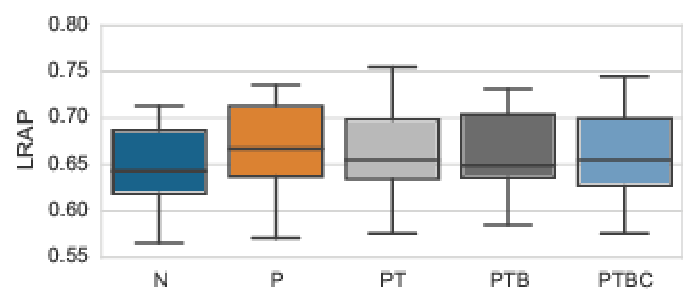
\includegraphics[width=\columnwidth]{figs/lrapall}
    \caption{Test-set score distributions (label-ranking average precision), aggregated
        across train-test splits.\label{lrapresults}}
\end{figure}

\Cref{lrapresults} illustrates the test-set performance aggregated across all splits. 
Because of the relatively small size of MedleyDB and the need for
artist-conditional splits, the resulting test-sets are small and thus exhibit high
variance across splits.  
As a basic sanity check, we first note that training with degraded audio does not appear
to decrease overall performance.
Between the no-augmentation condition (N) and pitch-shifting augmentation, there is a
small, but consistent improvement in performance.  A Wilcoxon signed-rank test between
conditions (N) and (P) produced a test statistic of 2018 and $p=2.25\times 10^{-6}$.
However, little differentiation was be observed among the different augmentation conditions.

%\begin{figure}
%    \centering
%    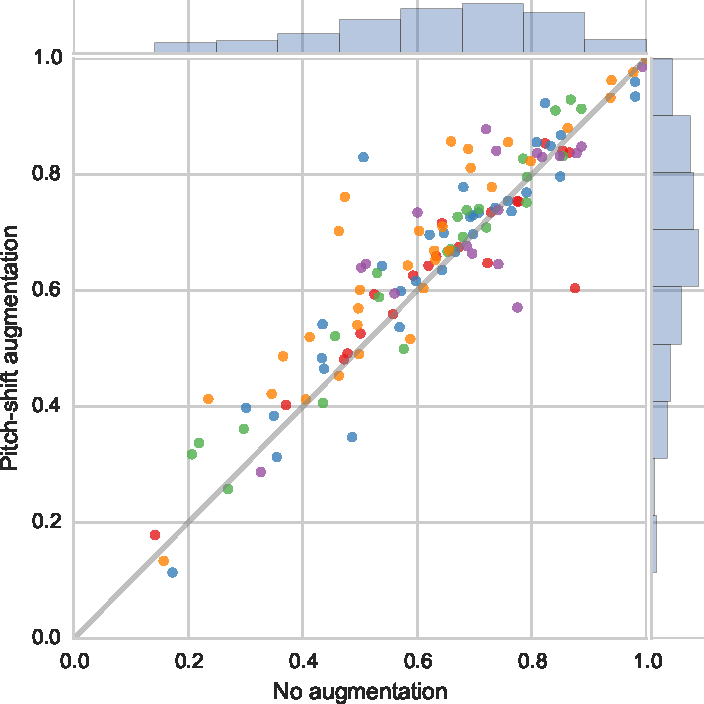
\includegraphics[width=0.75\columnwidth]{figs/onevstwo}
%    \caption{Point-wise comparison of test-set scores (LRAP)
%        for \emph{no augmentation} vs.\ \emph{pitch-shifting}.
%        Each point corresponds to a single test track.
%\label{onevstwo}}
%\end{figure}

%To more clearly investigate the effects of pitch-shifting augmentation, \Cref{onevstwo}
%illustrates the differences in accuracy between the no-augmentation models (N) and the
%models trained with additional pitch-shifted data (P), aggregated across all splits.
%The majority of test points lie above the main diagonal, indicating
%consistent improvements due to data augmentation.

\begin{figure}
    \centering
    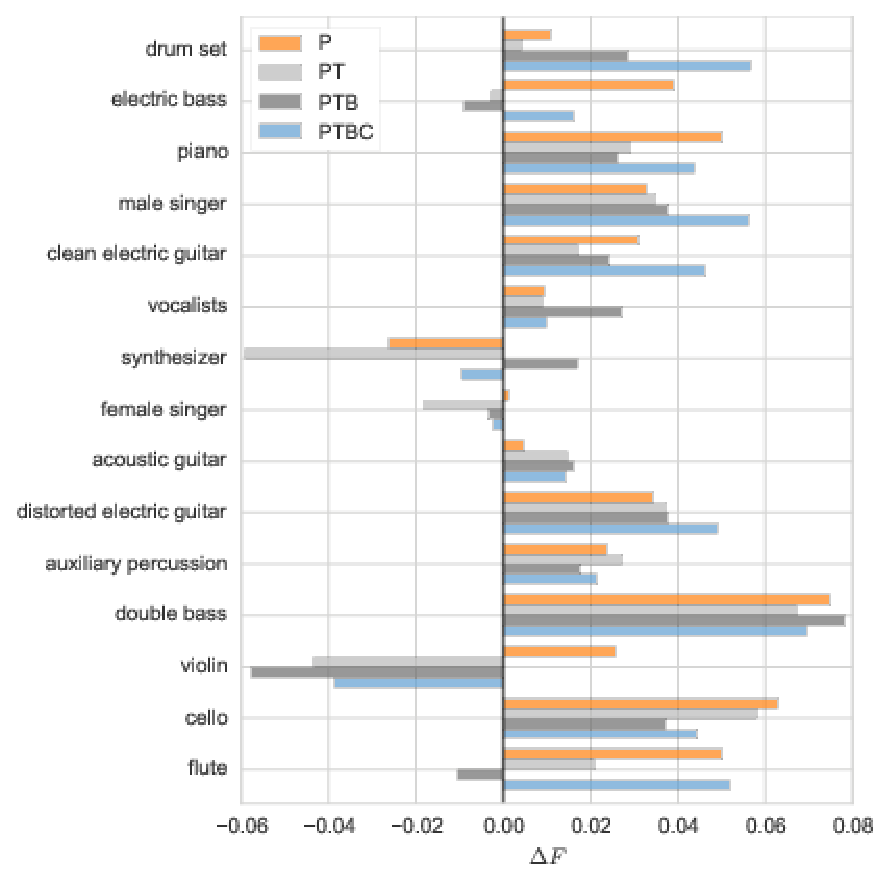
\includegraphics[width=\columnwidth]{figs/fscore-improvement}
    \caption{Per-class change in test-set $F$-score for each augmentation condition,
        relative to no-augmentation.  
        Positive changes indicate improvement by training with data augmentation.
        Results are averaged across splits.\label{fscore}}
\end{figure}

Next, we investigated the effects of data augmentation on each class.
\Cref{fscore} illustrates the change in per-class $F$-score relative to the
no-augmentation condition, averaged across across splits.
While the change varies between classes, the trend is generally positive
with the exceptions of \emph{female singer} and especially \emph{violin}.
In the latter case, negative change is only observed after introducing time-stretch
deformations, which may introduce unnatural distortions to the vibrato characteristics,
and thus make the class more difficult to model.

\section{Discussion}

% For bibtex users:

\bibliography{refs}

\end{document}
